\documentclass[tikz]{standalone}

\usepackage{amsmath}
\usepackage{unicode-math}
\usepackage{mathtools}
\usepackage{derivative}

\setmainfont{Stix Two Text}
\setmathfont{Stix Two Math}

\usetikzlibrary{arrows.meta,fit,positioning}

\renewcommand{\familydefault}{\sfdefault}

% prefix equation numbers with section number
\numberwithin{equation}{section}

\DeclarePairedDelimiter{\ceil}{\lceil}{\rceil}
\DeclarePairedDelimiter{\floor}{\lfloor}{\rfloor}
\DeclarePairedDelimiter{\abs}{\lvert}{\rvert}
\DeclarePairedDelimiter{\norm}{\lVert}{\rVert}
\DeclarePairedDelimiter{\bra}{\langle}{\rvert}
\DeclarePairedDelimiter{\ket}{\lvert}{\rangle}
\DeclarePairedDelimiter{\expval}{\langle}{\rangle}
\DeclarePairedDelimiter{\norder}{\mathcolon}{\mathcolon}
\DeclarePairedDelimiter{\anorder}{\typecolon}{\typecolon}
	
\newcommand{\laplace}{\mbfnabla^2}
\newcommand{\trans}{{\scriptscriptstyle\mathsf{T}}}

\newcommand{\vdot}{\cdot}
\newcommand{\vcross}{\vectimes}
\newcommand{\vb}[1]{\symbfup{#1}}
\newcommand{\vu}[1]{\hat{\vb{#1}}}
\newcommand*\dd[2][\relax]{\mathop{\ifx\relax#1\odif{#2}\else \odif[order={#1}]{#2}\fi\,}}

\newcommand{\vacuum}{\ket*{\vb{0}}}

\DeclareMathOperator{\trace}{Tr}
\DeclareMathOperator{\sinc}{sinc}

\AtBeginDocument{
	\let\Re\relax
	\let\Im\relax
	\DeclareMathOperator{\Re}{Re}
	\DeclareMathOperator{\Im}{Im}

	\renewcommand{\div}{\mathop{\mbfnabla\vdot}}
	\newcommand{\curl}{\mathop{\mbfnabla\vectimes}}
}

\DeclarePairedDelimiterX{\comm}[2]{[}{]}{#1,#2}

\DeclarePairedDelimiterX{\braket}[2]{\langle}{\rangle}{#1\delimsize\vert#2}
\DeclarePairedDelimiterX{\ketbra}[1]{\lvert}{\rvert}{#1\rangle\delimsize\langle#1}



\begin{document}
	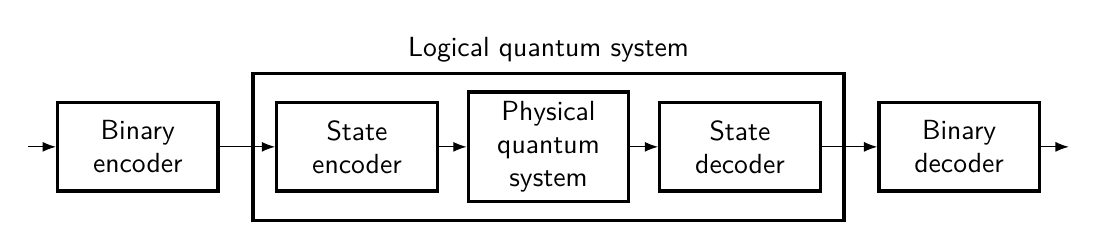
\begin{tikzpicture}[
		node distance=10pt,
		block/.style={draw, very thick, fill=white, minimum height=32pt, minimum width=58pt, text width=40pt, align=center},
		superblock/.style={draw, very thick, inner sep=8pt},
	]
		\node[block] (phy) {Physical quantum system};
		\node[block, left=of phy] (senc) {State encoder};
		\node[block, right=of phy] (sdec) {State decoder};
		\node[superblock, fit=(senc) (sdec), label={Logical quantum system}, inner xsep=8pt, inner ysep=10pt] (log) {};
		\node[block, left=20pt of senc] (benc) {Binary encoder};
		\node[block, right=20pt of sdec] (bdec) {Binary decoder};

		\coordinate[left=of benc] (in);
		\coordinate[right=of bdec] (out);
		
		\draw[-Latex] (in) -- (benc);
		\draw[-Latex] (benc) -- (senc);
		\draw[-Latex] (senc) -- (phy) ;
		\draw[-Latex] (phy) -- (sdec);
		\draw[-Latex] (sdec) -- (bdec);
		\draw[-Latex] (bdec) -- (out);
	\end{tikzpicture}
\end{document}
